%%%%%%%%%%%%%%%%%%%%%%%%%%%%%%%%%%%%%%%%%%%%%%%%%%%%%%%%%%%%%%%%%%%%%%
% amspaper.tex --  LaTeX-based template for submissions to American 
% Meteorological Society journals
%
% Template developed by Amy Hendrickson, 2013, TeXnology Inc., 
% amyh@texnology.com, http://www.texnology.com
% following earlier work by Brian Papa, American Meteorological Society
%
% Email questions to latex@ametsoc.org.
%
%%%%%%%%%%%%%%%%%%%%%%%%%%%%%%%%%%%%%%%%%%%%%%%%%%%%%%%%%%%%%%%%%%%%%
% PREAMBLE
%%%%%%%%%%%%%%%%%%%%%%%%%%%%%%%%%%%%%%%%%%%%%%%%%%%%%%%%%%%%%%%%%%%%%

%% Start with one of the following:
% DOUBLE-SPACED VERSION FOR SUBMISSION TO THE AMS
%\documentclass{ametsoc}

% TWO-COLUMN JOURNAL PAGE LAYOUT---FOR AUTHOR USE ONLY
\documentclass[twocol]{ametsoc}

%%%%%%%%%%%%%%%%%%%%%%%%%%%%%%%%
%%% To be entered only if twocol option is used

\journal{mwr}

%  Please choose a journal abbreviation to use above from the following list:
% 
%   jamc     (Journal of Applied Meteorology and Climatology)
%   jtech     (Journal of Atmospheric and Oceanic Technology)
%   jhm      (Journal of Hydrometeorology)
%   jpo     (Journal of Physical Oceanography)
%   jas      (Journal of Atmospheric Sciences)	
%   jcli      (Journal of Climate)
%   mwr      (Monthly Weather Review)
%   wcas      (Weather, Climate, and Society)
%   waf       (Weather and Forecasting)
%   bams (Bulletin of the American Meteorological Society)
%   ei    (Earth Interactions)

%%%%%%%%%%%%%%%%%%%%%%%%%%%%%%%%
%Citations should be of the form ``author year''  not ``author, year''
\bibpunct{(}{)}{;}{a}{}{,}

%%%%%%%%%%%%%%%%%%%%%%%%%%%%%%%%

%%% To be entered by author:

%% May use \\ to break lines in title:

%\title{A data-driven approach to parameterisations using convolutional encoder-decoder neural networks}
\title{On the potential for convolutional neural network approaches to inform parameterisations in numerical weather prediction models}
%%% Enter authors' names, as you see in this example:
%%% Use \correspondingauthor{} and \thanks{Current Affiliation:...}
%%% immediately following the appropriate author.
%%%
%%% Note that the \correspondingauthor{} command is NECESSARY.
%%% The \thanks{} commands are OPTIONAL.

\newcommand*\samethanks[1][\value{footnote}]{\footnotemark[#1]}

    \authors{Pablo Rozas Larraondo\correspondingauthor{Pablo Rozas Larraondo, 
     Fenner School of Environment \& Society, ANU Building 141, Linnaeus Way, Canberra, ACT, 2601}, Luigi Renzullo\thanks{Fenner School of Environment \& Society, ANU Building 141, Linnaeus Way, Canberra, ACT, 2601}, Jian Guo\thanks{National Computational Infrastructure, ANU Building 143, Ward Road, ACT, 2601, Australia}, I\~naki Inza\thanks{Intelligent Systems Group, Computer Science Faculty, University of the Basque Country UPV/EHU, Paseo de Manuel Lardizabal, Donostia, 20018, Spain} and Jose A. Lozano\footnotemark[3] \thanks{Basque Center for Applied Mathematics (BCAM), Mazarredo 14, Bilbao, 48009, Spain}}

     \affiliation{Fenner School of Environment \& Society, The Australian National University, Canberra, Australia}

\email{pablo.larraondo@anu.edu.au}


%%%%%%%%%%%%%%%%%%%%%%%%%%%%%%%%%%%%%%%%%%%%%%%%%%%%%%%%%%%%%%%%%%%%%
% ABSTRACT
%
% Enter your Abstract here

\abstract{Precipitation is one of the meteorological phenomena that has a great impact on human activities. The ability to accurately forecast precipitation is, therefore, an important task for current Numerical Weather Prediction (NWP) models. NWP precipitation is usually modelled using simplified or parameterised physical and chemical processes. The models representing these processes are often quite complex and require a high level of expertise in its design and tuning process. In this work, we devise a simple new methodology to derive precipitation from NWP geopotential fields using deep learning, a current hot-topic area of machine learning. Particularly, we consider a pipeline that first selects a set of geopotential height levels from the NWP and secondly uses these levels as the input to train three Convolutional Neural Network (CNN) models learning the precipitation field generated by the NWP. We include different experiments to compare the performance of each neural network as well as a comparison with alternative baseline machine learning methodologies. As far as we know, this paper covers the first attempt to model NWP parameterisations using generic machine learning methodologies.}

\iffalse
\abstract{NWP parameterisations use linear and non-linear models to approximate processes that are too small-scale or complex to be physically represented. Considerable effort and expertise are required to find good representations of atmospheric processes, and fine-tune the parameters. Artificial intelligence has recently achieved extraordinary results in image analysis using deep Convolutional Neural Networks (CNN). CNNs provide a generic methodology to characterize the structure of two-dimensional data, such as images or NWP gridded fields, finding relationships with a target function or field. In this article, we propose the use of CNN encoder-decoder architectures to compute derived NWP variables. Using ECMWF ERA-Interim data, we demonstrate how its total precipitation field can be reproduced with reasonable accuracy, using just the geopotential field as input. We compare different architectures and present a methodology to find the input variables which show the highest correlations. The CNN encoder-decoder models and techniques presented in this work are generic, and can be used to compute other parameterisations or for downscaling purposes.} 
\fi

\begin{document}


%% Necessary!
\maketitle


%%%%%%%%%%%%%%%%%%%%%%%%%%%%%%%%%%%%%%%%%%%%%%%%%%%%%%%%%%%%%%%%%%%%%
% MAIN BODY OF PAPER
%%%%%%%%%%%%%%%%%%%%%%%%%%%%%%%%%%%%%%%%%%%%%%%%%%%%%%%%%%%%%%%%%%%%%
%
\section{Introduction}

%Numerical Weather Prediction (NWP) is the foundation of most weather forecasting products nowadays. Many organisations across the planet dedicate significant amounts of compute power to simulate the evolution of the atmosphere by solving the primitive equations that govern its dynamics. However, there are physical processes occurring in the atmosphere, such as convection, friction or radiation, that cannot be represented succinctly by NWP, regardless of its resolution \citep{stensrud2009parameterization}. For these physical processes, NWP uses approximate models called parameterisations.

%NWP models resolve mid- and large-scale atmospheric processes under the assumptions of an adiabatic, frictionless atmosphere. Although these equations provide good approximations to the synoptic scale (i.e., $~\sim 1000$km) evolution of the atmosphere, exchanges of momentum, heat and moisture become important when simulating mid-range (36-72 hours) and sub-grid scale weather forecasts \citep{coiffier2011fundamentals}. NWP parameterisations make it possible to correctly account for the various dynamic and radiative processes in the atmosphere that influence the weather.

%Parameterisations, representing different atmospheric processes, are usually defined together inside "physical packages" that NWP models run \citep{LTG-81}. These parameterised processes interact with each other defining complex relationships. These relationships can be represented in the form of graphs, that often include feedback loops and nested dependencies. Often, a small modification in one of its parameters can lead to instabilities in  the NWP output. The process of designing and maintaining these "physical packages", which define the different parameterisations and their relationships, is laborious and requires a high level of expertise (i.e. human intervention).

%Although parameterisations based on statistical or probabilistic approaches -- mainly used for modelling turbulence -- can be found in the literature \citep{berner2017stochastic}, most of them are based on determistic model equations representing simplifications of the physical processes they try to encapsulate. In this paper, we propose a novel approach for defining NWP parameterisations in which the underlying physics, determining the relationships between atmospheric variables, can be learned as an optimisation problem using machine learning techniques.
Numerical Weather Prediction (NWP) underpins most weather forecasting services today. The steady increase of NWP skill over the last 40 year is inextricably linked to growth in computing power. Technological developments in computing have enabled finer-scale representation of physical processes in model simulations, facilitated the increased utilisation of earth observations (especially from satellites), and driven development of better methods of data assimilation (particularly ensemble methods), all of which contribute to the observed improved accuracy of NWP forecasts (Bauer et al, 2015). However, despite these technological advances, there remain physical processes, e.g. convection, friction or radiation, that cannot be adequately represented by NWP \citep{stensrud2009parameterization}. For these physical processes, NWP use model approximations called \emph{parameterisations}.

Parameterisations, typically representing sub-scale atmospheric processes, are usually lumped together inside "physical packages" that NWP models run \citep{LTG-81}. Most parameterisations are based on determistic model equations representing simplifications of the physical processes, however there are some that are statistical or probabilistic in form \citep{berner2017stochastic}. These parameterised processes can interact with each other leading to complex model behaviours.  Often, a small modification in one of the components of are can lead to inconsistencies with other parameterisations and ultimately results in instabilities in the NWP estimation. The process of designing and maintaining these "physical packages", which define the different parameterisations and relationships between them, is laborious and requires a high level of expertise, particularly human intervention.

((( Needs a paragraph introducing Machine Learning methods as having success in learning relationships from data without needing to specify the relayionships a priori  --- borrow from the next two paragraphs )))

%NWP models describe the state and evolution of the atmosphere, using a grid system that represents the spatial and temporal components of the output data, defining a highly structured space. The field of machine learning that studies structured domains is commonly known as "structured prediction" \citep{taskar2005learning}. Learning features on temporal and spatial dimensions are two common cases that structured prediction addresses \citep{gupta2010estimating,tran2012max}.

%One of the main limitations in applying traditional machine learning methods to NWP datasets has been the difficulty to accurately represent the spatial and temporal structure in the data. There are many examples in the literature applying supervised machine learning methods to improve the quality of NWP. These examples typically use observational data to downscale or correct bias and systematic errors in NWP \citep{loridan2017machine,gagne2014machine,foley2012current,rozas2014method}. The problem with these methods is that they are generally applied in isolation to individual, or small clusters of grid cells, without accounting for the surrounding spatial and temporal information present in the data. These approaches also often suffer from a lack of capacity to represent complex non-linear relationships in the data. 

%Spatial data analysis has received significant attention in machine learning. The problem of learning and analysing datasets that contain spatial features is commonly studied in the field of computer vision. For a long time, methods based on engineered features, such as SIFT \citep{lowe2004distinctive} and HOG \citep{dalal2005histograms} have been the standard approach for applying machine learning to images and other high-dimensional regular gridded data. In the last decade, new methodologies based on deep neural networks have been introduced, offering substantial advantages over previous approaches. 

Deep Learning \citep{lecun2015deep} methods have recently achieved unprecedented results in different supervised classification and regression tasks performed on different high dimensional datasets. These methods, based on the use of deep artificial neural networks, have surpassed human-level performance at different complex tasks such as image classification \citep{krizhevsky2012imagenet} or semantic description \citep{karpathy2015deep}. These architectures make use of Convolutional Neural Networks (CNN) \citep{krizhevsky2012imagenet}, which have been proven to be very effective at capturing intrinsic features represented at different scales of an image. CNNs arrange its neurons in three dimensions (width, height, depth) and establish local connections to capture the spatial features in the input image. These structures extract the spatial relationships on the data learning to represent features represented at different scale levels on images.

There has been a strong focus in the machine learning community to explore new methodologies that can be applied to large volumes of data. In particular deep learning \citep{lecun2015deep} methods have demonstrated state-of-the-art results using large data sets \citep{deng2009imagenet,openimages}. The application of these methodologies has also been explored in the field of weather forecasting with unprecedented results \citep{xingjian2015convolutional,liu2016application,rasp2018deep}.

Convolutional encoder-decoder networks are a type of CNN that provides state-of-the-art results at tasks such as image segmentation \citep{badrinarayanan2017segnet}, image denoising \citep{mao2016image} or image-to-image regression \citep{isola2017image}. These networks are based on autoencoders \citep{hinton2006reducing}, which use CNNs to learn reduced but accurate representations of images, generalising its use to find relationships between different images. Convolutions in the encoder half of the network perform a feature selection process by reducing the dimensionality of the data. The decoder part enlarges the feature space mapping it to the output space. Encoder-decoder networks offer an effective method for learning the relationship between high dimensional input and output spaces, such as the ones defined by images or video.

%Convolutional encoder-decoder networks have recently opened an active and promising field of research in areas such as medicine \citep{greenspan2016guest}, astronomy \citep{shallue2018identifying} or high-energy physics \citep{baldi2014searching}. In the field of weather and climate sciences there is also an incipient interest in the introduction of convolutional networks to perform analysis and interpretation of NWP weather and climate datasets \citep{liu2016application,xingjian2015convolutional,larraondo2017automating}.

In this work, we demonstrate how existing deep learning encoder-decoder networks, proposed in the field of image segmentation, can be adapted to perform regression tasks and learn NWP parameterisations using basic fields as input. Using the ERA-Interim geopotential height field as input, we demonstrate how encoder-decoder networks can learn to simulate non-trivial physical processes that relate this field to precipitation. The experimental section contains a comparison between the results obtained with deep encoder-decoder networks and traditional methodologies, such as random forest. The simplicity and effectiveness of this method constitutes an interesting alternative to the more complex parameterisation models currently used in NWP.

%We also propose a simple technique for quickly identifying the best set of input fields that produce the best results for a certain output field. This technique consist of using simplistic encoder-decoder decoder networks, which are fast to train, to iterate through all the different combinations in the input space to determine the relative contribution of each input field when predicting the output. In the experimental section, this technique is used to identify the geopotential heights in the atmosphere that show a higher correlation to the total precipitation field. These levels are then used to train the proposed deep encoder-decoder networks, which offer a significant improvement in accuracy when compared to the simplistic version. The performance and accuracy results of these networks are compared among themselves and also with alternative classic machine learning methods.

\section{Convolutional neural networks in the weather forecasting context}

The output of NWP are regular gridded numerical arrays representing physical parameters of the atmosphere over the spatial and temporal dimensions. 2-dimensional weather fields comprising the latitude and longitude dimensions are commonly represented as images, using colour palettes and superimposing maps to facilitate their interpretation by weather forecasters. In this section we introduce Convolutional Neural Networks (CNN), an image analysis methodology from the field of computer vision, and their applications to NWP interpretation and parameterisation problems.

Convolution, in the image processing context, is a mathematical operation performed over a group neighbour pixels of an image, weighted by a 2-dimensional matrix called kernel. The output of an image convolution is another transformed image with the same dimensions as the original image -- ignoring border effects. Performing an image convolution requires the application of the same operation iteratively, by sliding the kernel across the whole image. The result of each convolution operation is assigned to the pixel in the new image at the position designated by the kernel's centre.

Figure \ref{convolution_op} contains a representation of how a convolution operation is applied using a 3x3 kernel over a region of a gridded NWP 500 hPa geopotential field. The following equation shows the decomposed convolution operation between the different grid points in a region of a weather field \textbf{F}, a convolution kernel \textbf{K} and how the results are assigned to an output image \textbf{C}: 

\begin{equation}
c_{ij} = 
\begin{bmatrix}
    f_{i-1j-1} & f_{ij-1} & f_{i-1j+1} \\
    f_{i-1j} & f_{ij} & f_{ij+1}\\
    f_{i-1j+1} & f_{ij+1} & f_{i+1j+1}
\end{bmatrix}
\circledast
\begin{bmatrix}
    k_{11} & k_{12} & k_{13}\\
    k_{21} & k_{22} & k_{23}\\
    k_{31} & k_{32} & k_{33}
\end{bmatrix}
=

    f_{i-1j-1} \cdot k_{11} + f_{ij-1} \cdot k_{12} + f_{i-1j+1} \cdot k_{13} + f_{i-1j} \cdot k_{21} + & f_{ij} \cdot k_{22} +  f_{ij+1} \cdot k_{23} + f_{i-1j+1} \cdot k_{31} + f_{ij+1} \cdot k_{32} + f_{i+1j+1} \cdot k_{33}

\end{equation}

\begin{figure*}[h]
 \centerline{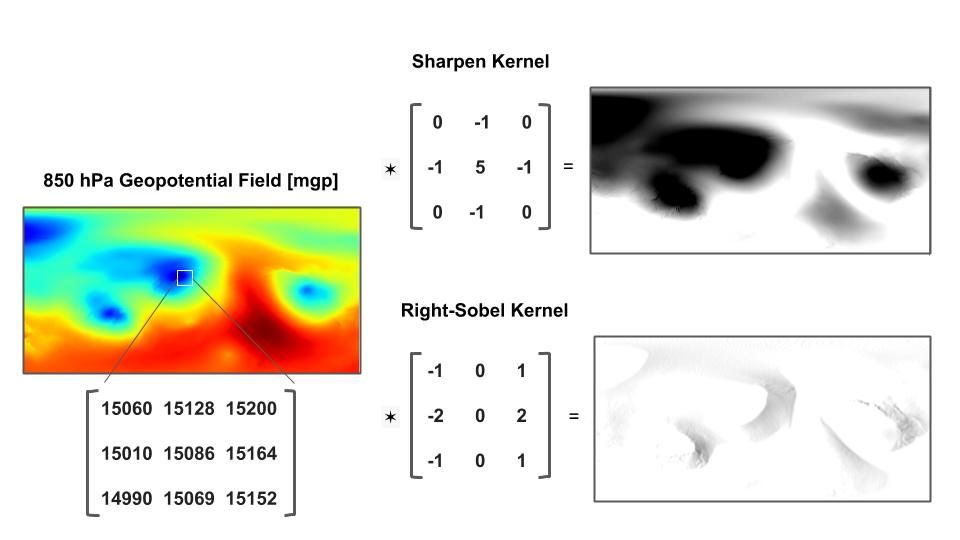
\includegraphics[width=10cm]{convolution_op.png}}
  \caption{Graphical representation of the experiment pipeline comprising the variable selection and the encoder-decoder network comparison processes.}\label{convolution_op}
\end{figure*}

Different kernels perform different transformations in the output image, such as image sharpening, blurring or edge detection. Figure \ref{kernels} shows the effect of two different convolution kernels on a 500hPa geopotential height field. In this figure we can see how the sharpen kernel has the effect of highlighting the regions of the image that present larger gradients. The right-sobel kernel, on the other hand, detects the edges with an orientation to the right or, in other words, it makes salient the regions of the image that contain right to left decreasing gradients. Detecting the regions with certain gradient configurations can be intuitively related to the activity of drawing fronts in geopotential height maps, which are normally used to identify precipitation regions. 

\begin{figure*}[h]
 \centerline{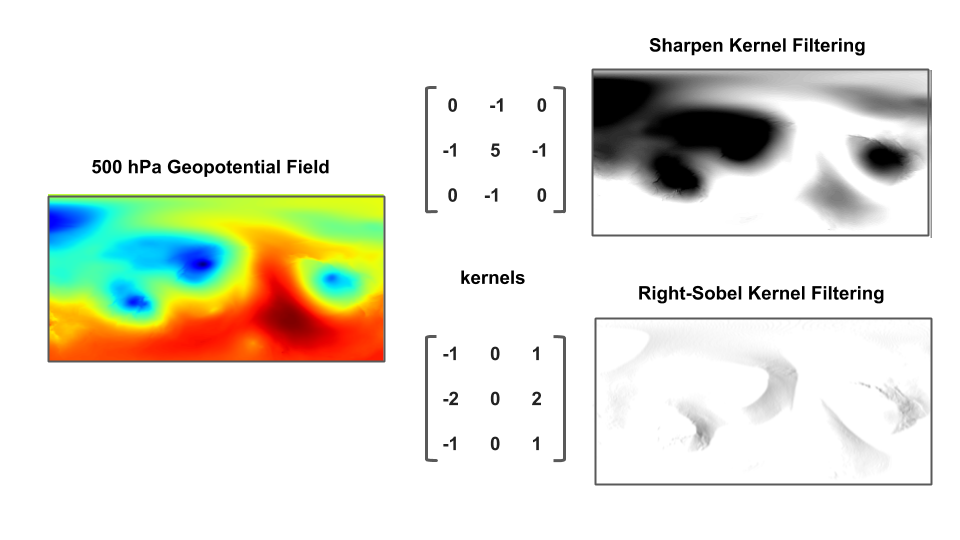
\includegraphics[width=10cm]{kernels.png}}
  \caption{Graphical representation of the experiment pipeline comprising the variable selection and the encoder-decoder network comparison processes.}\label{kernels}
\end{figure*}

Convolutions can be applied to Objectively, this convolution kernel could potentially be used as an automated method to identify the regions of the atmosphere that present a sudden increase in the geopotential height field following the zonal flow of the atmosphere.

Convolutional Neural Networks (CNN) \citep{lecun2010convolutional}, are a particular type of feed-forward artificial neural network, which is specifically designed to perform image classification and regression tasks. These networks consist on a series of consecutive layers which perform convolution operations extracting the spatial information of input images. Instead of using predefined kernels, CNNs use gradient descent \citep{bottou2010large} to find the optimal kernels by reducing an error function that meassures the accuracy of a task during training. The network learns, during the training process, the weights that transform a series of input images into a close representation of their corresponding outputs.

The convolution operations, at each layer of a CNN, are commonly followed by an operation that causes a reduction in the size of the image, and an activation function \citep{glorot2010understanding}. The dimensionality reduction is usually achieved by applying a specific subsampling method called pooling \citep{scherer2010evaluation} or by performing the convolution operation on strides over the image. The convolution, pooling and non-linear activation function, performed at each layer of a CNN, result in a gradual reduction in the size of the input image, which implies that kernels can cover increasingly larger areas relative to the initial image. This characteristic allows CNNs to identify features at different scales in an image. Fig \ref{cnn_scales} represents the reduction in the size of a NWP geopotential height field performed by a 4 layers CNN. Each pooling operation in this network reduces the size of the image to a half. As the dimensions of the image decrease, each grid point represents a larger area and kernels are able to extract mesoscale and synoptic scale features in the initial image. 

\begin{figure*}[h]
 \centerline{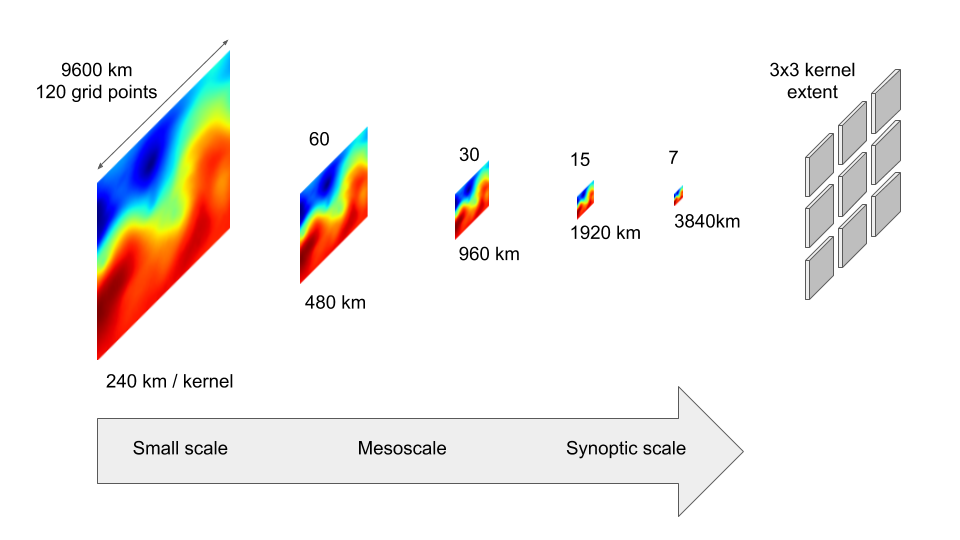
\includegraphics[width=10cm]{cnn_scales.png}}
  \caption{Graphical representation of the experiment pipeline comprising the variable selection and the encoder-decoder network comparison processes.}\label{cnn_scales}
\end{figure*}

Convolutions, on each layer of a CNN, transform the dimensionality of the input image reducing its spatial extent and expanding, at the same time, the number of features along a third dimensional axis. This expansion of the image shape along the third dimension reases the information by the image at each layer of the network, in which different layers encode different relationships in the image. This expansion in depth of the images is achieved using 3-dimensional kernels, in which 2-dimensional kernels are stacked and each one individually learns to detect specific patterns in the image.

CNNs have been applied to solve many classification and regression tasks in different fields, such as medical image analysis \citep{litjens2017survey}, high-energy physics \citep{baldi2014searching} or astronomy \citep{dieleman2015rotation}. CNNs have demonstrated to be an effective approach in which similar architectures can be trained to perform different tasks.

Autoencoders \citep{hinton2006reducing} are a type of neural networks that can learn to create compressed representations of the input data. These networks perform a dimensionality reduction followed by an expansion of the input space trained to recreate the original input. Convolutional autoencoders \citep{masci2011stacked} use CNNs to learn compressed representations of images. Convolutional encoder-decoder networks use convolutional layers to compress, or reduce the dimensionality of input images, followed by deconvolutional layers, which perform the inverse operation by expanding the dimension of the data. These two parts define a symetrical structure in which the first half receives the name of encoder and the second half is the decoder. Convolutional encoder-decoder networks have been mainly used to perform image segmentation tasks, in which the network has to identify parts of an image belonging to the same class \citep{long2015fully}.

Image segmentation using convolutional encoder-decoder networks has been an active area of research in recent years \citep{krizhevsky2012imagenet,chen2018deeplab}. Several techniques and network architectures have been proposed to improve the accuracy of the image segmenting process. The main constraint of convolutional encoder-decoder networks is the loss of spatial information, caused by dimensionality reduction pooling operations \citep{scherer2010evaluation}. A consequence of this is that output images lack resolution and features often become blurry or ill defined. Many convolutional encoder-decoder network architectures have been proposed to mitigate the loss of spatial information: Segnet \citep{badrinarayanan2017segnet} uses the transferred pool indices from its encoder to communicate the exact pixel position to the decoder. U-net \citep{ronneberger2015u}, on the other hand, enables precise localization by creating connections between the symmetric convolution and deconvolution operations to capture spatial context.

A generalisation of convolutional encoder-decoder networks is found in pixel-to-pixel regression or image-to-image translation networks \citep{isola2017image}. Existing networks used in to perform image segmentation can be applied to regression problems by replacing the network's loss function by a regression one, such as Root Mean Square Error (RMSE) or Mean Absolute Error (MAE).

NWPs simulate a large number of physical variables with different levels or dependence. Some of these variables are derived from other fields using physical equations or parameterisation models. Convolutional encoder-decoder networks provide a generic methodology to perform regression between different weather fields. These networks can therefore be used to learn the underlying relationships between NWP fields. In the next section we explore the use of CNNs to learn NWP parameterisations using basic fields as input.

For this work, we use the NWP ERA-Interim \citep{dee2011era} global climate reanalysis dataset produced by the European Centre for Medium-Range Weather Forecasts (ECMWF). This dataset contains data from 1979 every 6 hours to present. The spatial resolution of the data set is approximately 80 km (reduced Gaussian grid N128) on 60 vertical levels from the surface up to 0.1 hPa. ERA-Interim data is publicly accessible from ECMWF's Public Datasets web interface \citep{1321008426928}.

ERA-Interim makes available a large number of output parameters, from which we choose geopotential height \textit{(\textbf{z})} and total precipitation \textit{(\textbf{tp})}. The experiments in the next section train models that can learn to predict total precipitation using geopotential height fields as the only input.

We crop an extended area over Europe (\textit{latitude: [75, 15], longitude = [-50, 40]}), and select a subset of geopotential heights \textit{(\textbf{z})} at the following pressure levels of the atmosphere: [1000, 900, 800, 700, 600, 500, 400, 300, 200, 100] hPa. The resulting geopotential height data are stored as a 4-dimensional numerical array with shape [54.023, 10, 80, 120] for the corresponding dimensions [time, height, latitude, longitude]. 

% tp already defined above, thus deleted text.
The ERA-Interim \textit{(\textbf{tp})} parameter represents the total amount of precipitation accumulated at each grid point during a 3-hour period measured in metres (1000 litres/squared metre). This field is aggregated to match the 6-hour frequency of the geopotential height field by adding 2 consecutive lead-time accumulations and scaled by 1,000 to represent millimetres (1 litre/squared metre) of rain. The result is a 3-dimensional numerical array with shape [54.023, 80, 120] for the corresponding dimensions [time, latitude, longitude]. Figure \ref{dataset} represents the geographic area as well as the correspondence between the geopotential height and the total precipitation field time series. 

\begin{figure*}[h]
 \centerline{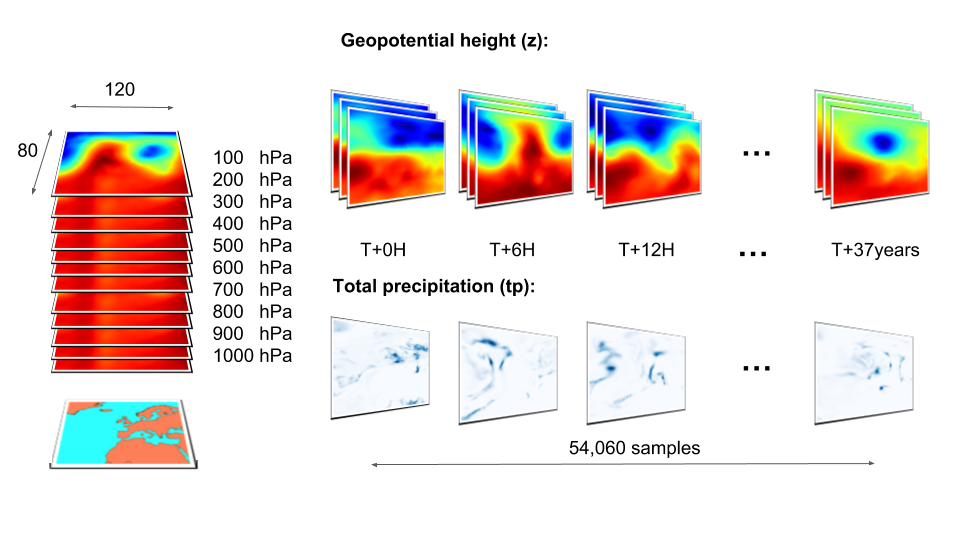
\includegraphics[width=13cm]{dataset.png}}
  \caption{Representation of the geographic area covered by the dataset and the geopotential height and total precipitation temporal series.}\label{dataset}
\end{figure*}

\subsection{Methodology}

NWP parameterisations of cloud and precipitation processes make simplifying assumptions, either for the purpose of computational efficiency or due to the uncertainty associated with these individual processes, in particular micro-physics and sub-grid scale interactions \citep{lopez2007cloud}. These parameterisations, depending on their nature, are classified in two groups: deterministic or probabilistic. 

Deterministic parameterisations are commonly found in NWP \citep{kain2004kain,tiedtke1989comprehensive}, based on the definition of new physical models or approximations to describe atmospheric processes. Both linear and non-linear regression are used to define parameterisations \citep{crawford1999improved,feng20073}. 

Probabilistic parameterisations use statistical methods by means of stochastic dynamic equations \citep{berner2017stochastic}. This area represents a novel and promising field of research for improving the quantification of NWP uncertainty or generating variability in ensemble based NWP.

An alternative approach is to consider parameterisations as a learning process using supervised machine learning methodologies to find the relationships between different variables, given a large enough dataset of historical records. Machine learning offers a broad collection of methodologies, such as random forests \citep{breiman2001random}, support vector regression or neural networks that can solve generic regression problems. However, the application of these techniques is rarely found in the NWP parameterisation literature, apart from a few examples \citep{lipponen2013correction}.

As mentioned in the introduction, the output of NWP defines an structured data set along the temporal and spatial dimensions. NWP datasets present a challenge for traditional machine learning methodologies because of their high dimensionality and volume. 

Computer vision is a field of machine learning that applies algorithms to perform different tasks on high dimensional datasets, such as digital images. Common problems addressed in this field are image denoising, segmentation, upsampling or detection of objects. Algorithms in this area use a broad range of approaches based on the application of geometry, statistical or physical models. 

Image classification, used in applications such as face detection or object detection, maps the high dimensional space of an image into a category \citep{haralick1973textural} or value \citep{takeda2007kernel} that identifies the contents of the image. A more challenging problem is to map one image to another, because the dimensionality of the output space makes it very difficult for machine learning algorithms to find relationships between both spaces. Image segmentation is a common image-to-image classification problem that assigns a label to each pixel in an image to determine the boundaries of objects in the image. Image segmentation algorithms apply different methods such as logistic regression, support vector machines or random forests to images for classifying its pixels \citep{haralick1985image,pal1993review,pal2005random}. Image denoising and upsampling are examples of image-to-image regression, in which the task consists in learning to predict the numerical values of each pixel in the output image, as opposed to a categorical value in image segmentation problems. This is a much harder problem than image-to-image classification and algorithms in this area normally include different forms of neighbour embedding to provide context for each pixel, using principal component analysis or random forests \citep{chang2004super,schulter2015fast}.

Convolutional Neural Networks (CNN) \citep{lecun2010convolutional}, are a particular type of feed-forward artificial neural networks specifically designed to analyse images. The application of fully-connected neural networks to high-dimensional data, such as images, has failed because of the large number of connections required to map the input space into the network. CNNs propose a simplified model in which neurons in one layer connect only to a local region of the next layer. This region is called kernel and its weights are shared across the image for each layer of the CNN, which results in translation invariance characteristics \citep{scherer2010evaluation}. These kernels define a limited area in the width and height dimensions of an image but comprise the total depth dimension of images, which usually corresponds to the Red, Green and Blue (RGB) channels of a colour image. The convolution operation performs a cross-correlation operation by sliding the kernel across the image. The weights of the kernel are updated during training using backpropagation \citep{widrow199030} to minimise the error of a given loss function. 

Autoencoders \citep{hinton2006reducing} are generic neural networks that reproduce the input by performing a dimensionality reduction and subsequent expansion of the input space. This technique allows learning compressed representations of the data in an unsupervised manner. Convolutional autoencoders \citep{masci2011stacked} use CNNs to learn compressed representations of images. Convolutional encoder-decoder networks are a latter evolution of convolutional autoencoders which can perform image segmentation tasks, by mapping an input image to an output segmented image \citep{long2015fully}.

Image segmentation using convolutional encoder-decoder networks has been an active area of research in recent years \citep{krizhevsky2012imagenet,chen2018deeplab}. Several techniques and network architectures have been proposed to improve the accuracy of the image segmenting process. The main constraint of convolutional encoder-decoder networks is the loss of spatial information, caused by dimensionality reduction pooling operations \citep{scherer2010evaluation}. A consequence of this is that output images lack resolution and features often become blurry or ill defined. Many convolutional encoder-decoder network architectures have been proposed to mitigate the loss of spatial information: Segnet \citep{badrinarayanan2017segnet} uses the transferred pool indices from its encoder to communicate the exact pixel position to the decoder. U-net \citep{ronneberger2015u}, on the other hand, enables precise localization by creating connections between the symmetric convolution and deconvolution operations to capture spatial context. 

A generalisation of convolutional encoder-decoder networks is found in pixel-to-pixel regression or image-to-image translation networks \citep{isola2017image}. Existing segmentation networks can be easily modified to perform image-to-image translation tasks by substituting the classification loss function by a regression one, such as Root Mean Square Error (RMSE) or Mean Absolute Error (MAE).

Although most of the research on CNNs has been performed using colour images as input, the same networks have been proven to be effective with other types of image data, such as multispectral images in the fields of remote sensing \citep{hu2015transferring} or volumetric medical imaging \citep{milletari2016v}. In weather forecasting, NWPs produce gridded outputs representing physical parameters for different vertical levels of the atmosphere. In this paper we propose the use of NWP fields as input channels for CNNs, combining them to analyse and interpret weather data.

The experimental section in this paper explores the application of convolutional encoder-decoder segmentation networks adapted to perform grid to grid regression (image to image regression) and learn NWP parameterisations directly from basic atmospheric fields. Specifically, we demonstrate how the total precipitation field can be learned, per grid point, using geopotential height as the only input.


\section{Experimental design}

The objective of the experiments presented in this work is to demonstrate that convolutional encoder-decoder neural networks can be used, as an alternative to NWP parameterisations, to learn complex atmospheric processes, such as precipitation, using basic NWP fields as input.

Geopotential height is closely related with air pressure and is one of the most fundamental physical variables used in weather forecasting. This field is simulated by NWP models by solving the primitive equations of the atmosphere. Geopotential height has been traditionally used by weather forecasters to detect fronts, which separate masses of air of different properties, and ultimately forecast the occurrence and intensity of precipitation \citep{renard1965experiments,hope2014comparison}.

Existing NWP precipitation parameterisations normally use geopotential height in combination with other basic variables, such as temperature, humidity or vorticity as inputs. For this work we propose the use of geopotential height at different levels as the only input variable to forecast total precipitation for the following reasons: 1. Using a low number of inputs simplifies the encoder-decoder model and results in faster training process. 2. It demonstrates the ability of neural networks to find complex non-linear relationships between input and output grid fields that are not obviously correlated. 3. It serves as a nod to the hundreds of skilled human weather forecasters that are able to provide an accurate analysis using this field exclusively.

To perform the comparison between the different encoder-decoder models, we propose the use of a pipeline comprising two steps. The first step performs a variable selection process to determine the geopotential height levels that minimise the error at forecasting the total precipitation field. The second step compares the results of three state-of-the-art convolutional encoder-decoder architectures, in the field of image segmentation, at learning to predict the ERA-Interim total precipitation field.

The input dataset comprises ten levels of the geopotential height; however, due to the linear increase in the number of trainable parameters and the hardware requirements to train these convolutional encoder-decoder networks, we limit the number of input levels to three. Different methods for performing variable selection have been proposed \citep{saeys2007review}. These methods generally reduce the search space of input variables and optimise the construction of accurate predictors. 

For our experiment, we build a simplified convolutional encoder-decoder network and perform an exhaustive search using all the different combinations of 1, 2 and 3 elements, out of the 10 geopotential field levels. The combination that reaches the lower error is chosen. 

This simplified network has a similar architecture to the deeper encoder-decoder networks, but its complexity is reduced by limiting the number of layers and depth of the convolution operations. Performing a similar exhaustive search of  input variables with the deeper, more complex networks, like the ones introduced in the next part of the experimental process, would be computationally infeasible. However, this simplified network allows a quick iteration across the whole feature space to identify the subset of geopotential heights that minimises the error of the precipitation field in the training set.

To identify the levels of geopotential height that produce the best precipitation results, the simple convolutional encoder-decoder network is trained with all the different combinations of the ten levels, without repetition. Therefore, the number of models that need to be trained is:

\begin{equation}
C_1(10) + C_2(10) + C_3(10) = \binom{10}{1} + \binom{10}{2} + \binom{10}{3} = 175
\end{equation}

This process requires training the same network 175 times using the different combinations of the input data. The results of this variable selection process are used to compare the accuracy of the three state-of-the-art deep encoder-decoder convolutional networks in the second step of the pipeline. Therefore, the final validation comparing the accuracy of the different networks must be performed using a different dataset partition that remains unseen during the variable selection process  \citep{reunanen2003overfitting}.

\begin{figure*}[h]
 \centerline{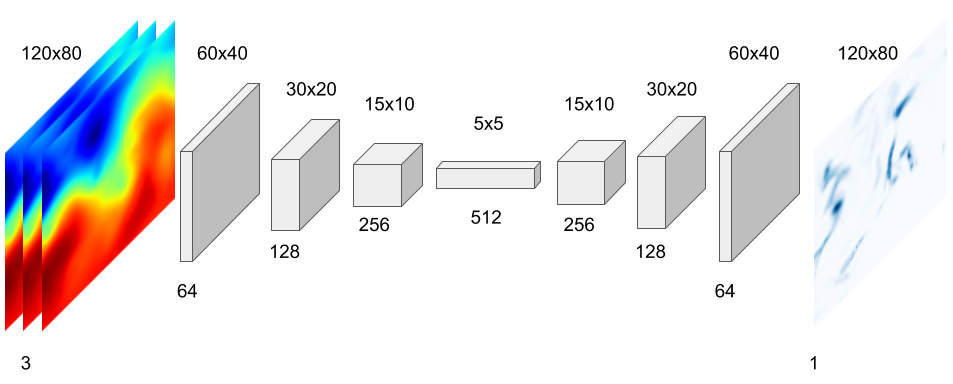
\includegraphics[width=13cm]{vgg16_enc.png}}
  \caption{Transformations in the dimensionality of the data performed by a VGG-16 encoder-decoder to map between the input and output spaces.}\label{vgg16}
\end{figure*}

The whole pipeline can be seen as a variable selection process followed by the neural network model comparison process. The initial dataset, which contains 54,060 samples, is randomly split into the training and validation datasets, containing 80\% and 20\% of the data respectively, so that there is an even proportion of the different meteorological situations in both splits. These partitions are used to evaluate the differences in accuracy between the compared deep architectures. The variable selection process is performed internally using the training dataset, which is further split into 80\% and 20\% partitions to train and validate the different subsets of input variables. The final comparison between the architectures is performed using the initial 20\% validation split, which does not intervene at neither the variable selection process nor the training of the different architectures. Figure \ref{exp} represents the proposed experiment and the relationship between the variable selection the model evaluation processes. 

\begin{figure*}[h]
 \centerline{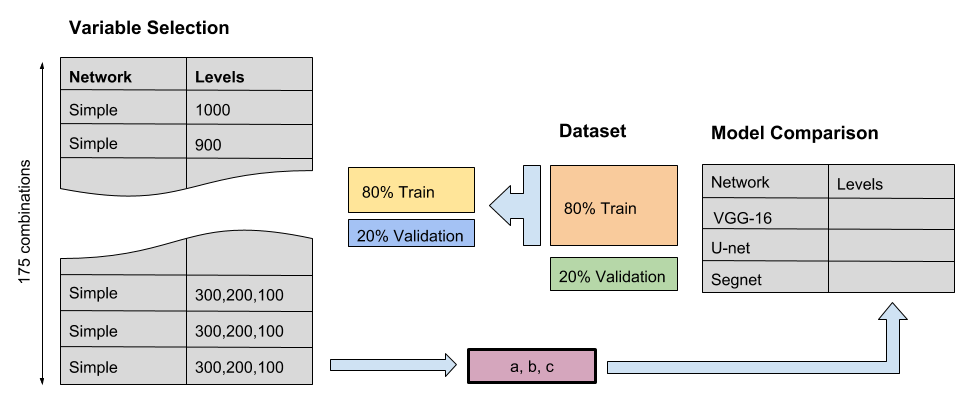
\includegraphics[width=13cm]{experiment.png}}
  \caption{Graphical representation of the experiment pipeline comprising the variable selection and the encoder-decoder network comparison processes.}\label{exp}
\end{figure*}

The network used for to perform the variable selection process is a simplification of the VGG-16 convolutional encoder-decoder network \citep{long2015fully}, which has demonstrated state-of-the-art results in image segmentation tasks. Figure~\ref{vgg16} represents the dimensionality transformations performed by the VGG-16 network to the input space using 3x3 convolutions using stride value of 2 to perform the spatial dimension reduction. The simplification proposed for this part of the experiment is to remove the last convolution operation in the encoder section. The information gets compressed to a depth of 256 channels instead of the 512 in the full VGG-16 network. This simplified network reduces significantly the total number of parameters when compared to the full VGG-16 which results in a significant reduction in the amount of compute resources required to train it. Each network is trained during 20 epochs (iterations over the internal input training split) and their results are honestly computed using the MAE metric comparing the predicted outputs to the total precipitation field in the internal validation dataset. The results of this first experiment are therefore used to determine the geopotential height levels that minimise the error at forecasting total precipitation. 

The second step of the pipeline focuses on finding which deep encoder-decoder convolutional network is more accurate at forecasting ERA-Interim's total precipitation field. For this part, we use the levels of geopotential height, computed previously, to compare the three different state-of-the-art segmentation networks.

We consider three different state-of-the-art convolutional encoder-decoder networks in the field of image segmentation: VGG-16 \citep{long2015fully}, Segnet \citep{badrinarayanan2017segnet} and U-net \citep{ronneberger2015u}. These networks are modified to perform regression tasks instead of classification by changing the loss function to MAE. To accomplish an honest comparison between these three networks, we build them using the same number of layers and depth of the convolution operations. The basic structure for all three networks is represented in Figure~\ref{vgg16}. Therefore, all three networks perform the same dimensionality transformations when estimating total precipitation from the geopotential height input. The difference between these networks resides in the number of convolution operations performed at each layer and in the configuration of the connections between layers. VGG-16 presents a linear architecture, in which each layer is only connected to the adjacent ones. Segnet computes the index of the max pooling operation at each of the encoder layers and communicates this value to its symmetric in the decoder, so they can be used in the up-sampling stage. The U-net decoder, on the other hand, concatenates the weights used in the encoder part to reconstruct the spatial information. The objective of this second half of the experimental process is to determine the network that provides the best accuracy when forecasting total precipitation.

All three networks are trained using the initial 80/20 split defined at the beginning of the experiment. This way, the validation split used to compare the accuracy of the different networks has remained unseen during at the variable selection and training of the different networks. This method assures the independence and fairness of the results between both experiments. 

The networks are trained during 50 epochs using the subset of geopotential heights selected in the first part of the experiment as input and the total precipitation field as output. The same optimiser (stochastic gradient descent), learning rate (0.01) and loss function (MAE) as in the variable selection process are used to train the three networks. These networks are then compared with the total precipitation field in the validation split dataset produced by ERA-Interim, to determine the error.

The models are implemented using the Keras \citep{chollet2017keras} framework and the TensorFlow \citep{abadi2016tensorflow} back-end. These models, as well as a copy of the dataset used in the experiments, are available at this repository: \url{https://github.com/prl900/precip-encoder-decoders}.

\section{Results and discussion}

\subsection{Variable selection process}

In the first part of the experiment we identify the levels of the geopotential height that produce a better estimate in the training set of the ERA-Interim total precipitation field. We train the simple encoder-decoder network 175 times as described in the previous section using the training split. 

The resulting models are then compared using the internal validation split, which is formed with the remaining 20\% of the initial training split. The MAE metric is used to compare the error in predicting total precipitation at each point of the grid. Figure \ref{heatmap} contains the MAE scores produced for each combination of any two geopotential height levels compared to the total precipitation field produced by the NWP. The results indicate that combinations of lower levels of the atmosphere produce better estimates of the precipitation field than the higher levels. The main diagonal of the matrix in Figure \ref{heatmap} represents the resulting errors when using a single geopotential level to train the network. Individually, the lower levels of the atmosphere present lower MAE values when forecasting precipitation, being 900 hPa the one with the lowest error. In the case of using two inputs, the lowest errors are found when combining low and mid levels of geopotential, being the combination of 1000 and 500 hPa levels the one with the lowest error.

\begin{figure}[h]
 \centerline{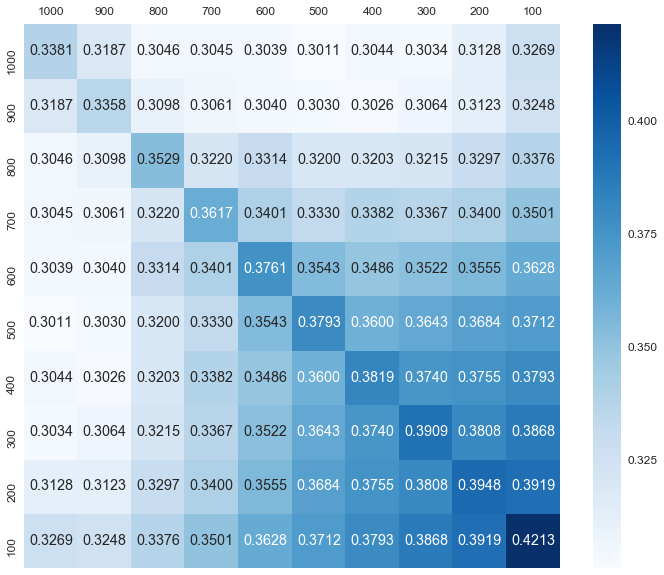
\includegraphics[width=8cm]{heatmap.png}}
  \caption{Matrix representing the average validation MAE results for each simple encoder-decoder network trained with each possible combination of two geopotential levels.}\label{heatmap}
\end{figure}

Training the encoder-decoder network with three geopotential levels, results in a significant improvement in performance. Table \ref{3leveltable} contains the five lowest error results and their corresponding atmospheric levels. Unfortunately, the results for three levels cannot be easily represented graphically. Compared to the previous results, there is a significant improvement in performance when a third level is added as input to the encoder-decoder network. This implies that the neural network is capable of finding internal relationships between the different levels of the atmosphere and relate them with precipitation events. The combination of 1000, 800 and 400 hPa geopotential heights results in the lowest error of the total precipitation field in the training partition. This result is surprisingly similar to the traditional practice in weather forecasting of using the sea-level, 850 and 500 hPa geopotential fields to determine the location of weather fronts and therefore, precipitation. 

\begin{table}[h]
\caption{Top 5 average MAE results when training the simple encoder-decoder network with every combination of three geopotential height levels to predict the ERA-Interim total precipitation field.}\label{3leveltable}
\begin{center}
\begin{tabular}{cc}
\topline
$z\hspace{1em}levels$ & $MAE$\\
\midline
 1000, 800, 400 & 0.2895 \\
 1000, 800, 500 & 0.2897 \\
 1000, 900, 500 & 0.2897 \\
 1000, 900, 400 & 0.2901 \\
 1000, 700, 400 & 0.2927 \\
\botline
\end{tabular}
\end{center}
\end{table}

The MAE values represented in Table \ref{3leveltable} are calculated using the average of the MAE results over the 120 by 80 grid area and for all the temporal entries in the validation dataset. Considering that the total precipitation field is expressed in millimetres, the error of these networks when forecasting total precipitation is, on average, less than 1/3th of litre per square metre in a 6-hour period, when compared to the values produced by the NWP.

\subsection{Deep convolutional networks' comparison}

For this part of the experimental process, we choose the subset of 1000, 800 and 400 hPa geopotential heights to evaluate the performance of deeper, state-of-the-art segmentation encoder-decoder networks adapted to perform regression tasks. The number of parameters and depth of these networks is significantly higher than the simplified network previously used to perform the selection of the geopotential levels. Training these deeper networks demands therefore significantly higher compute and memory resources, we use a compute node equipped with a Tesla P100-PCIE-16GB accelerator provided by the Australian National Computational Infrastructure.

Table \ref{perftable} represents the total number of trainable parameters for each of these networks and the total amount of time required to train the different networks during 50 iterations (epochs) over the initial training split. The total number of trainable parameters provides an indication of the size of each network and the time value in this table gives an indication of the time required to train each network using TensorFlow models running on a P-100 NVIDIA GPU node.

\begin{table}[h]
\caption{Number of parameters for each encoder-decoder network architectures and resulting training time for each network (50 epochs).}\label{perftable}
\begin{center}
\begin{tabular}{crc}
\topline
$Network$ & $Parameters$ & $Time\ [hours]$\\
\midline
 Simple (ref.) & 745,000 & 0.6 \\
 VGG-16 & 16,467,469 & 4.7 \\
 U-net & 7,858,445 & 2.4 \\
 Segnet & 29,458,957 & 8.6 \\
\botline
\end{tabular}
\end{center}
\end{table}

Figure \ref{training} shows the learning process of the four different encoder-decoder networks during 50 iterations (epochs) over the training dataset. At the end of each epoch during training, the validation dataset is used to assess the error of the model and the improvement of the different models can be honestly compared using unseen data. At the beginning of the training process the network learns fast and it slows down as the training progresses. The reduction in the validation error is different for each network which flattens at different points and rates.

\begin{figure}[h]
 \centerline{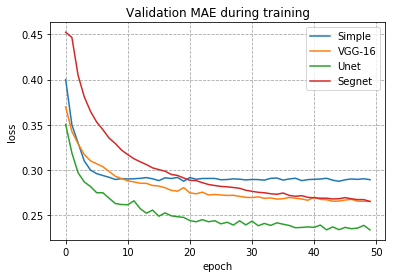
\includegraphics[width=8cm]{training.png}}
  \caption{Comparison of the evolution of the validation error during training for the four convolutional encoder-decoder networks over 50 epochs.}\label{training}
\end{figure}

\begin{figure*}[h]
 \centerline{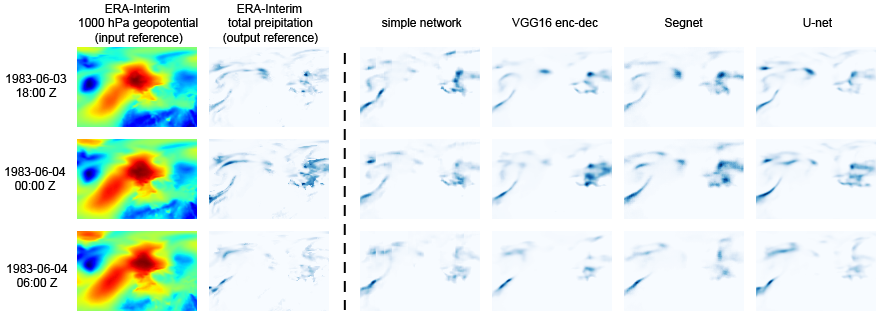
\includegraphics[width=17cm]{comparison.png}}
  \caption{Visual comparison between the total precipitation field generated by the different networks. ERA-Interim 1000 hPa geopotential height and total precipitation fields are included for reference.}\label{comparison}
\end{figure*}

\begin{table}[h]
\caption{Accuracy of the different networks using the validation split at the end of the training process.}\label{deep_results}
\begin{center}
\begin{tabular}{cl}
\topline
$Network$ & $MAE$\ [mm]\\
\midline
 Simple & 0.2893 \\
 VGG16 & 0.2630 \\
 Segnet & 0.2618 \\
 U-net & 0.2386 \\
\botline
\end{tabular}
\end{center}
\end{table}

Considering the validation results in Figure \ref{training} and the size of each network in Table \ref{perftable}, we highlight the behavior of U-net which shows the lowest validation error and is also the one with the lowest number of parameters of the three deep learning networks considered. 

Figure \ref{comparison} offers a visual comparison between the outputs generated by each model for an atypical atmospheric situation around the 15th of June of 1983. The first two columns from the left represent the 1000 hPa geopotential height and total precipitation, as produced by the ERA-Interim model. Total precipitation represents the total precipitation accumulated over the 6-hour period following the indicated time. In a similar way, and using the same colour scale, the next 4 columns represent the precipitation generated by the different encoder-decoder networks.

The spatial structure and intensity of the precipitation field is represented differently by each network, with slight variations in respect of the ERA-Interim reference output. Different convolutional encoder-decoder networks use different methods to reconstruct the spatial information lost during the encoding phase. Apart from capturing the spatial structure of the precipitation field, the different networks have to provide accurate results for the precipitation intensity at each grid point.

\subsection{Statistical analysis of the results}
To compare the performance of the different convolutional encoder-decoder architectures we use the validation split to extract the total precipitation at the closest grid point to nine different cities produced by each network. Figure \ref{cities} represents the geographical location of these nine cities within the region of our dataset. These cities are located in different climatic zones and present distinct precipitation patterns.

\begin{figure}[h]
 \centerline{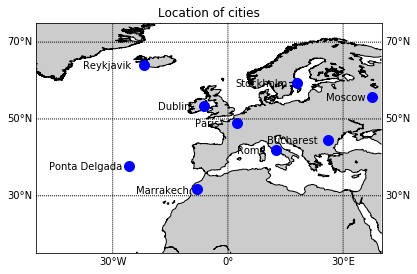
\includegraphics[width=8cm]{cities.png}}
  \caption{Location of the nine different cities within the comprised region.}\label{cities}
\end{figure}

Results are assessed using the ERA-Interim total precipitation field as reference for the same grid points using the signed error -- or bias -- metric. This metric provides information about possible biases and distribution of the error as opposed to the previously used MAE, which does not provide information about the sign of the error. For each city and point in time the error in predicting total precipitation is calculated. These results are then aggregated by city and type of network. Figure \ref{violin} uses a violin plot \citep{hintze1998violin} to represent the error results at each location for the different architectures. A violin plot proposes a modification to box plots adding the density distribution information to the basic summary statistics inherent in box plots. The horizontal blue bar towards the centre of each of the violins in Figure \ref{violin}, represents the mean. The lower part in each plot, shows the mean $(\mu)$ and standard deviation $(\sigma)$ of the error values for each network and location. The shape of the violin gives a visual indication of each model's performance. Wider and sharper violin shapes around the 0 value provide an indication of good network performance.

\begin{figure*}[h]
 \centerline{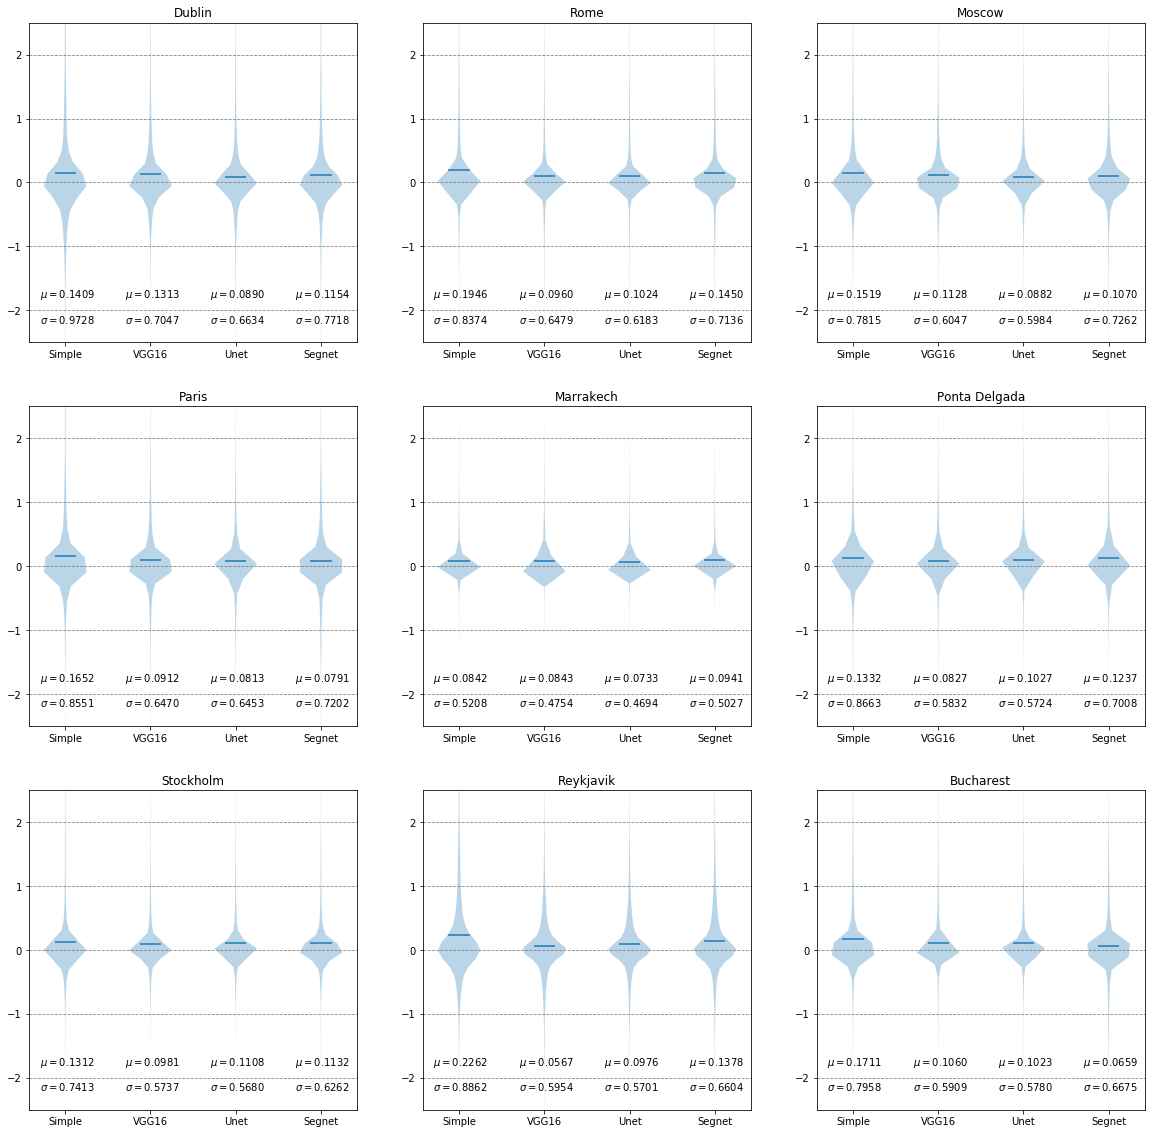
\includegraphics[width=16cm]{violin.png}}
  \caption{Representation of the error density function and the mean $(\mu)$ and standard deviation $(\sigma)$ values for the different architectures at each city.}\label{violin}
\end{figure*}

In order to statistically compare the results, we use the methodology proposed by Demsar \citep{demsar2006} to assess the statistical significance of the differences between the error results of each network in the nine locations. The initial Friedman test rejects the null hypothesis of similarity among the 4 convolutional encoder-decoder networks. This justifies the use of post-hoc bivariate tests, Nemenyi \citep{pohlert2014pairwise} our case, to assess the significance of the differences between the different pairs of encoder-decoder networks. 

The results of these tests are graphically expressed using Critical Difference (CD) diagrams. The Nemenyi test pairwisely compares the error results between any two architectures. Differences are considered significant if the corresponding average rank differs by at least one critical difference.

\begin{figure}[h]
 \centerline{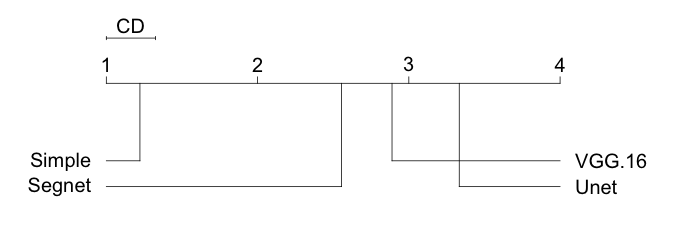
\includegraphics[width=8cm]{CD.png}}
  \caption{Critical Differences comparing the 4 convolutional encoder-decoder architectures. $\alpha = 0.05$ }\label{CD}
\end{figure}

Figure \ref{CD} shows a CD diagram representing the results of the Nemenyi test $(\alpha = 0.05)$ using the error values at the nine locations for each convolutional encoder-decoder network. 

CD diagrams make a pairwise comparison between methods, connecting the architectures for which no significant statistical differences are found, or in other words, those whose distance is less than the fixed critical difference, shown at the top of Figure \ref{CD}. Networks ranked with lower values in CD diagrams imply higher error values. These tests have been performed using the \texttt{scmamp} R package, which is publicly available at the Comprehensive R Archive Network (CRAN) \citep{calvo2015}. 

Statistical differences are found between all pairs of networks. As can be seen in the CD diagram, the performance of U-net is significantly better at forecasting total precipitation than the other 3 networks. VGG-16 and Segnet have a significantly lower performance but they are still considerably better than the simple convolutional encoder-decoder described in the first part of the experimental process. These results imply that U-net based architectures provide better results when forecasting total precipitation, using geopotential height as input. Considering the results presented in Table \ref{perftable}, U-net requires approximately half the GPU and memory resources than VGG-16 or a quarter than Segnet equivalent networks.

\subsection{Comparison with traditional methods}

This section is intended to provide readers with an understanding of the qualitative improvement that deep convolutional architectures offer when compared to previous machine learning methodologies.

First of all, we provide a baseline comparison of precipitation forecast using persistence. We consider two different constant rain fields using zero and the average precipitation over the area of study. This two situations represent the cases where we always predict that there is no precipitation or the average precipitation based on the climatology at each grid point. The MAE results of comparing these two scenarios to the ERA-Interim precipitation values over the validation dataset are represented in Table \ref{persistence}.

\begin{table}[h]
\caption{Baseline comparison of precipitation forecast using constant values over the whole area.}\label{persistence}
\begin{center}
\begin{tabular}{ll}
\topline
$Constant\ value\ [mm]$ & $MAE$\ [mm]\\
\midline
 0 (No precipitation) & 0.3417 \\
 0.45 (Mean precipitation) & 0.4845 \\
\botline
\end{tabular}
\end{center}
\end{table}

The results in Table \ref{persistence} indicate that forecasting no precipitation provides a substantially better forecast than using the average value. The mean in this case  results in a poor estimate for the precipitation field. The distribution of precipitation has a high variability, precipitations concentrates around well defined clusters and in most of the grid points there is no precipitation. This is why using zero precipitation performs better than the mean value for the MAE metric.

A common technique in computer vision is to train model that learn to predict the value of a pixel using a patch containing the surrounding pixels in the input space \citep{pal2005random,mueller2016water}.
We approach the problem of learning the total precipitation field from the 3 levels of geopotential height determined previously, but using traditional regression methodologies. We choose three common regression algorithms: linear regression, Least Absolute Shrinkage and Selection Operator (LASSO) and random forest regressor. Due to the high dimensionality of the data, we train the different algorithms using increasingly larger patches (1,3,5,7 and 9) comprising the 3 levels in the input to predict the central pixel in the output.

As the size of the patch increases the overlap area between two adjacent patches is larger and the size of the dataset increases and the resulting dataset cannot fit in memory of high-end machines. To train the different models we randomly sample 100.000 patches of each size.

Table \ref{regress} contain the MAE results of the different regression models for each patch size. Looking at the results, it can be concluded that none of these techniques is capable of learning the relationships between the geopotential and total precipitation fields of a NWP. Also, because these models are trained using a narrow patch or window of the input field, they cannot even match the accuracy of the naive approaches proposed at the beginning of this section.

Figure \ref{reg_comp} shows the output generated by each regression algorithm for the same meteorological situation presented in Figure \ref{comparison}. The models are not able to provide the sharpness necessary to represent the precipitation field. I can be seen that the output generated by Random forest provides a light improvement in detecting the position of the precipitation regions, possibly because is the only non-linear method. However, the capacity of this methodology is not enough to resolve this problem.

\begin{table}[h]
\caption{Comparison of the accuracy level for the different regression models.}\label{regress}
\begin{center}
\begin{tabular}{lccccc}
\topline
$method$ & \multicolumn{5}{c}{patch size}\\
\midline
 & 1 & 3 & 5 & 7 & 9\\
\midline
 Lin.\ Reg. & 0.5281  & 0.5061  & 0.5055  & 0.5054  & 0.5105 \\
 LASSO & 0.5281 & 0.5056 & 0.5049 & 0.5034 & 0.5034\\
 RF & 0.5437 & 0.4924 & 0.4903 & 0.4862 & 0.4851\\
\botline
\end{tabular}
\end{center}
\end{table}

\begin{figure*}[h]
 \centerline{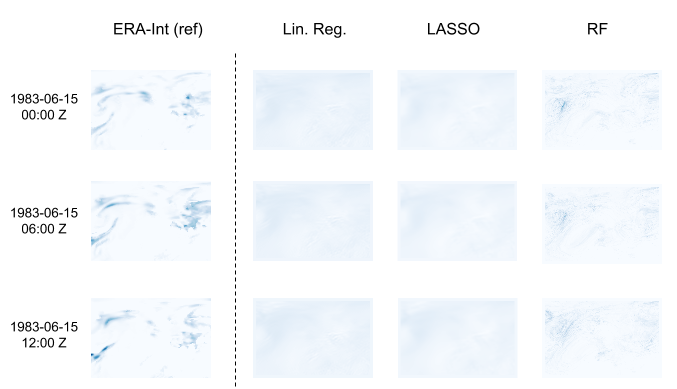
\includegraphics[width=16cm]{baseline.png}}
  \caption{Output of the three regression methods (patch size = 7) using the same dates shown in Figure 6.}\label{reg_comp}
\end{figure*}
\section{Conclusions and future work}

This work demonstrates the suitability of convolutional encoder-decoder networks in learning NWP parameterisations using only the geopotential height field to predict total precipitation. Considering the results presented in this manuscript, it is noticeable that the geopotential height at different levels of the atmosphere contains enough information to infer the precipitation field, as shown in Figures \ref{comparison} and \ref{violin}. There are many other physical variables simulated by NWP, such as temperature or humidity, that contain valuable information to determine the location and intensity of precipitation. Although adding these variables as inputs to the encoder-decoder convolutional networks improves significantly the accuracy of the precipitation results, this paper focuses on demonstrating the capacity of these networks to find relationships between different variables. The spatial structures at different levels of the atmosphere of the geopotential field contains enough information to estimate a precipitation field with reasonable accuracy.

The networks presented in the experimental section of this paper uses a loss function to train the models based on the mean absolute error metric. Verification of NWP precipitation, can be based on a wide variety of metrics. For example, there are effects such as the 'Double Penalty' \citep{mass2002does,bougeault2003wgne} that become important when atmospheric structures are correctly represented in terms of their shape and intensity but not in their position. We consider that further research on defining new loss functions based on existing verification methods, that can account for errors in the spatial structure \citep{rossa2008overview}, would lead to more accurate parameterisation models.

In this work we present a model that is trained to output precipitation values from the geopotential field. The quality of our model is therefore limited by the quality of the underlying NWP parameterisation used to simulate precipitation. The same encoder-decoder network could ideally be trained using observed precipitation data, resulting in a better model. Unfortunately, the research community has currently no access to observational datasets that match the spatial and temporal resolution of NWP. However, the rapid evolution of satellite and earth observation technologies open the possibility of having new high quality observations at a global scale in the future.

Lastly, another promising evolution of the methodology presented here, is to modify the convolutional encoder-decoder networks introducing recurrent structures. Recurrent neural networks \citep{mikolov2010recurrent} have demonstrated remarkable results in the area of time-series analysis and speech recognition and they open an interesting new line of research for models that can learn from both the spatial and temporal components of NWP data.

%%%%%%%%%%%%%%%%%%%%%%%%%%%%%%%%%%%%%%%%%%%%%%%%%%%%%%%%%%%%%%%%%%%%%
% ACKNOWLEDGMENTS
%%%%%%%%%%%%%%%%%%%%%%%%%%%%%%%%%%%%%%%%%%%%%%%%%%%%%%%%%%%%%%%%%%%%%
\acknowledgments

We would like to thank the National Computational Infrastructure (NCI) at the Australian National University and the University of the Basque Country for their support and advice in carrying out this research work.

We are grateful for the support of the Basque Government (IT609-13), the Spanish Ministry of Economy and Competitiveness (TIN2016-78365-R). 

Jose A. Lozano is also supported by BERC program 2014-2017 (Basque Gov.) and Severo Ochoa Program SEV-2013-0323 (Spanish Ministry of Economy and Competitiveness).

%%%%%%%%%%%%%%%%%%%%%%%%%%%%%%%%%%%%%%%%%%%%%%%%%%%%%%%%%%%%%%%%%%%%%
% REFERENCES
%%%%%%%%%%%%%%%%%%%%%%%%%%%%%%%%%%%%%%%%%%%%%%%%%%%%%%%%%%%%%%%%%%%%%


 \bibliographystyle{ametsoc2014}
 \bibliography{references}

\end{document}
%%%%%%%%%%%%%%%%%%%%%%%%%%%%%%%%%%%%%%%%%%%%%%%%%%%%%%%%%%%%%%%%%%%%%
% END OF AMSPAPER.TEX
%%%%%%%%%%%%%%%%%%%%%%%%%%%%%%%%%%%%%%%%%%%%%%%%%%%%%%%%%%%%%%%%%%%%%
%%%%%%%%%%%%%%%%%%%%%%%%%%%%%%%%%%%%%%%%%%%%%%%%%%%%%%%%%%%%%%%%%%%%%%
% amspaper.tex --  LaTeX-based template for submissions to American 
% Meteorological Society journals
%%%%%%%%%%%%%%%%%%%%%%%%%%%%%%%%%%%%%%%%%%%%%%%%%%%%%%%%%%%%%%%%%%%%%%
% amspaper.tex --  LaTeX-based template for submissions to American 
% Meteorological Society journals
